% !TeX encoding = UTF-8
% !TeX spellcheck = en_US
% !TeX root = 1315LectureNotes.tex
\chapter{Solutions Bound in Sets}\label{chap:numAndSets}
\begin{genericFrame}[frametitle={~New Things\hbox{~}}]
    \textbf{\Large\sffamily Definitions}
    \begin{description}[style=nextline]
        \item[Set] a collection of items
        \item[Element of set \(A\)] An item inside the set \(A\). If
         \(x\) is an element of the set \(A\), then we write
         \(x\in A\). Otherwise, we write \(x\notin A\) to say that the
         item \(x\) is not an element of \(A\).
        \item[Empty Set] the unique set which has nothing inside it,
         i.e. no elements. We write \(\emptyset\) to mean the empty 
         set.
        \item[Real Numbers] the set which contains all integers,
         fractions, and irrational numbers. We write \(\reals\) to
         mean the real numbers, or more properly, the set of real
         numbers.
    \end{description}
    \textbf{\Large\sffamily Notation}
    \begin{itemize}
        \item Roster Method for describing a set
        \item Set-Builder Method for describing a set
    \end{itemize}
\end{genericFrame}

\section{Sets Contain Solutions}
\subsection{Definition}\label{sec:set_defn}
A \textbf{set} is simply a container, albeit an abstract container, of 
various items. When we talk about a specific set, lets just use an 
arbitrary set \(A\) as an example, the items contained inside this set 
\(A\) are called the \textbf{elements} of this set. When talking about 
a specific item, say \(x\) for example, we will write \(x\in A\) to 
mean that the item \(x\) is an element of the set \(A\). Likewise, we 
write \(x\notin A\) to mean that \(x\) is not an element of \(A\).

\subsection{Naming Sets}
We need to have some examples of the kind of sets that we'll be working
with in this class. There are two ways of naming, or describing, a set.

\subsubsection{Roster Method}
Here is one such example.
\[\set{2, 3, 5, 7}\]
This is the set that contains the numbers 2, 3, 5, and 7, and no other
elements. The method of writing a set in this way is known as the
\textbf{roster method}. It's most convenient when dealing with sets 
that have a small number of elements.

\subsubsection{Set-Builder Method}
But we will be dealing with sets that have infinitely many members. For
these sets, we describe them using \textbf{Set-Builder method}.
\[\set{x\mid x\lt 5} \text{read: the set of all element \(x\) such %
    that \(x\) is less than 5}\]

It starts, and ends, with the same curly braces \(\set{}\), describes
the type of elements it contains, e.g. a single number represented by
\(x\), and gives a condition which determine whether or not an item is
a member in the set, e.g. \(x\lt 5\). For our set above, if any single
number, represented by \(x\), is less than 5, then \(x\) is an element
of this. And every element of our set must be numbers less than 5.
Another way to represent this set is with a number line.

\begin{center}
	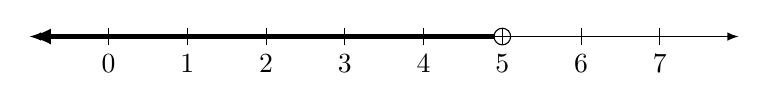
\begin{tikzpicture}
		\draw[latex-,ultra thick] (-1,0) -- (5, 0);
		\draw[fill=white] (5,0) circle (3pt);
		\draw[latex-latex] (-1,0) -- (8, 0);
		\foreach \x in {0, 1, 2, 3, 4, 5, 6, 7}
			\draw[shift={(\x,0)}] (0, 3pt) -- (0, -3pt);
		\foreach \x in {0, 1, 2, 3, 4, 5, 6, 7}
			\draw[shift={(\x,0)}] (0,-3pt) node[below] {\(\x\)};
	\end{tikzpicture}
\end{center}

\section{Sets in College Algebra}
The other common types of sets we will encounter are the set of all 
real numbers \(\mathbb{R}\), and the empty set \(\emptyset\), which is 
the set that contains nothing at all.